% =====================================================================
% manuscript.tex  —  the paper.
%
% GOLDEN RULE (see CLAUDE.md §8): no number in this file is typed by hand.
%   * tables come in via \input{tables/*.tex}
%   * figures via \includegraphics{figures/*.pdf}
%   * in-text numbers via macros defined in tables/estimates.tex
%     (e.g. \betaAbs, \lambdaAbs), which code/02_analyze.py regenerates.
% To change a number, change the code and re-run `python code/run_all.py`.
% =====================================================================
\documentclass[11pt]{article}

\usepackage[margin=1in]{geometry}
\usepackage{amsmath}
\usepackage{booktabs}
\usepackage{graphicx}
\usepackage[round]{natbib}
\usepackage[hidelinks]{hyperref}

\graphicspath{{figures/}}
% Auto-generated by code/02_analyze.py — DO NOT EDIT BY HAND.
% Each macro is a number the manuscript cites in prose (CLAUDE.md §8).
\newcommand{\startYear}{1960}
\newcommand{\finalYear}{2019}
\newcommand{\horizon}{59}
\newcommand{\Nabs}{105}
\newcommand{\betaAbs}{-0.0017}
\newcommand{\seAbs}{0.0012}
\newcommand{\pAbs}{0.165}
\newcommand{\rsqAbs}{0.016}
\newcommand{\lambdaAbs}{0.17}
\newcommand{\halflifeAbs}{397}
\newcommand{\sigmaStart}{1.018}
\newcommand{\sigmaEnd}{1.214}
\newcommand{\sigmaSlope}{0.0039}
\newcommand{\Nsigma}{105}
   % defines \betaAbs, \lambdaAbs, \sigmaStart, ...

\title{Testing the Convergence Prediction of the Solow Model\\
       with the Penn World Table}
\author{QuaRCS Lab \\ \small An AI-assisted, fully reproducible example}
\date{\today}

\begin{document}
\maketitle

\begin{abstract}
The Solow growth model predicts that economies converge to their steady states,
so that poorer economies should grow faster and catch up. We test this using the
Penn World Table 11.0 for \Nabs{} economies over \startYear--\finalYear. We find
\emph{no} evidence of \emph{absolute} convergence: the cross-country relationship
between initial income and subsequent growth is weak and statistically
insignificant ($\beta = \betaAbs$, $p = \pAbs$), implying a convergence speed of
only $\lambdaAbs\%$ per year. Consistent with this, cross-country dispersion of
income did not fall but \emph{rose} over the period (the standard deviation of
log GDP per capita moved from \sigmaStart{} to \sigmaEnd). The Solow model,
however, predicts convergence only after conditioning on determinants of the
steady state; we take up that conditional test in ongoing work.
\end{abstract}

\section{Introduction}
\label{sec:intro}
A central prediction of the neoclassical growth model \citep{solow1956} is
\emph{convergence}: because of diminishing returns to capital, an economy that
starts further below its steady state grows faster. Whether this catch-up is
visible in the data has been one of the most studied questions in empirical
macroeconomics \citep{barro1991, barrosala1992, mrw1992}. A useful distinction is
between \emph{$\beta$-convergence} --- a negative relationship between initial
income and subsequent growth --- and \emph{$\sigma$-convergence} --- a decline
over time in the cross-country dispersion of income \citep{barrosala2004}.

This paper is a compact, fully reproducible test of these predictions using the
latest Penn World Table \citep{feenstra2015}. Every number, table, and figure in
this document is emitted by the code in \texttt{code/} and pulled in
automatically; nothing is transcribed by hand. The point is as much the
\emph{workflow} --- a verifiable, AI-assisted research pipeline --- as the
economics.

\section{Data}
\label{sec:data}
We use the Penn World Table version 11.0 \citep{feenstra2015}, which reports real
national-accounts output in constant 2021 US dollars. Our income measure is real
GDP per capita, \texttt{rgdpna/pop}. We take a long growth window,
\startYear--\finalYear, ending before the COVID-19 disruption. Table~\ref{tab:attrition}
documents how the estimation sample is built from the raw panel; every excluded
economy is accounted for. Table~\ref{tab:summary} reports summary statistics.

% Auto-generated by code/ — DO NOT EDIT BY HAND.
\begin{table}[htbp]
\centering
\caption{Sample construction and attrition.}
\label{tab:attrition}
\begin{tabular}{llll}
\toprule
Stage & Criterion & Countries & Dropped \\
\midrule
0 & PWT 11.0: all economies & 185 &  \\
1 & GDP p.c. observed and positive in 1960 & 111 & 74 \\
2 & GDP p.c. observed and positive in 2019 & 111 & 0 \\
3 & Not a PPP outlier at either endpoint & 105 & 6 \\
4 & Solow controls present (conditional sample) & 99 & 6 \\
\bottomrule
\end{tabular}
\\[2pt]
\footnotesize Income per capita is rgdpna/pop from PWT 11.0 (2021 US\$). The conditional sample (stage 4) additionally requires the Solow controls (investment share, population growth, human capital).
\end{table}

% Auto-generated by code/ — DO NOT EDIT BY HAND.
\begin{table}[htbp]
\centering
\caption{Summary statistics (country cross-section).}
\label{tab:summary}
\begin{tabular}{llllll}
\toprule
Variable & count & mean & std & min & max \\
\midrule
Log GDP p.c., initial & 105 & 8.305 & 1.018 & 5.727 & 10.59 \\
Log GDP p.c., final & 105 & 9.49 & 1.214 & 6.916 & 11.623 \\
Avg. annual growth & 105 & 0.02 & 0.014 & -0.018 & 0.062 \\
Investment share & 105 & 0.214 & 0.083 & 0.071 & 0.459 \\
Population growth & 105 & 0.018 & 0.009 & 0.001 & 0.042 \\
Depreciation rate & 105 & 0.043 & 0.012 & 0.016 & 0.09 \\
Human capital & 99 & 2.073 & 0.635 & 1.071 & 3.407 \\
\bottomrule
\end{tabular}
\end{table}


\section{Methods}
\label{sec:methods}
Let $y_{i,t} = \ln(\text{GDP per capita})$ and let $T = \horizon$ be the length
of the window. We measure average annual growth as
$g_i = (y_{i,\finalYear} - y_{i,\startYear})/T$. \emph{Absolute} $\beta$-convergence
is the cross-country regression
\begin{equation}
  g_i = \alpha + \beta\, y_{i,\startYear} + \varepsilon_i,
  \label{eq:absolute}
\end{equation}
estimated by OLS with heteroskedasticity-robust (HC1) standard errors;
convergence requires $\beta < 0$. The implied speed of convergence follows from
the Solow linearization, $\lambda = -\ln(1 + \beta T)/T$, with half-life
$\ln 2/\lambda$. For \emph{$\sigma$-convergence} we compute, on a balanced panel,
the cross-country standard deviation of $y_{i,t}$ in each year and test whether it
trends down.

\section{Results}
\label{sec:results}
Table~\ref{tab:convergence} reports the absolute $\beta$-convergence regression.
The estimated coefficient is $\betaAbs$ (robust s.e.\ $\seAbs$) and is not
statistically significant ($p = \pAbs$); the regression explains only a trivial
share of the variation in growth ($R^2 = \rsqAbs$). Taken at face value, the
implied convergence speed is just $\lambdaAbs\%$ per year --- economically
negligible. Figure~\ref{fig:beta} shows why: across the \Nabs{} economies there
is essentially no relationship between initial income and subsequent growth.

% Auto-generated by code/02_analyze.py — DO NOT EDIT BY HAND.
\begin{table}[htbp]
\centering
\caption{Beta-convergence of real GDP per capita, 1960--2019. Dependent variable: average annual log growth. Heteroskedasticity-robust (HC1) standard errors in parentheses.}
\label{tab:convergence}
\begin{tabular}{lc}
\toprule
 & Absolute \\
\midrule
Log initial GDP p.c. ($\beta$) & -0.0017 \\
 & (0.0012) \\
Constant & 0.0339*** \\
 & (0.0107) \\
\midrule
Implied $\lambda$ (\%/yr) & 0.17 \\
Half-life (yrs) & 397 \\
Observations & 105 \\
$R^2$ & 0.016 \\
\bottomrule
\end{tabular}
\\[2pt]
\footnotesize $^{*}p<0.1$, $^{**}p<0.05$, $^{***}p<0.01$.
\end{table}


\begin{figure}[htbp]
  \centering
  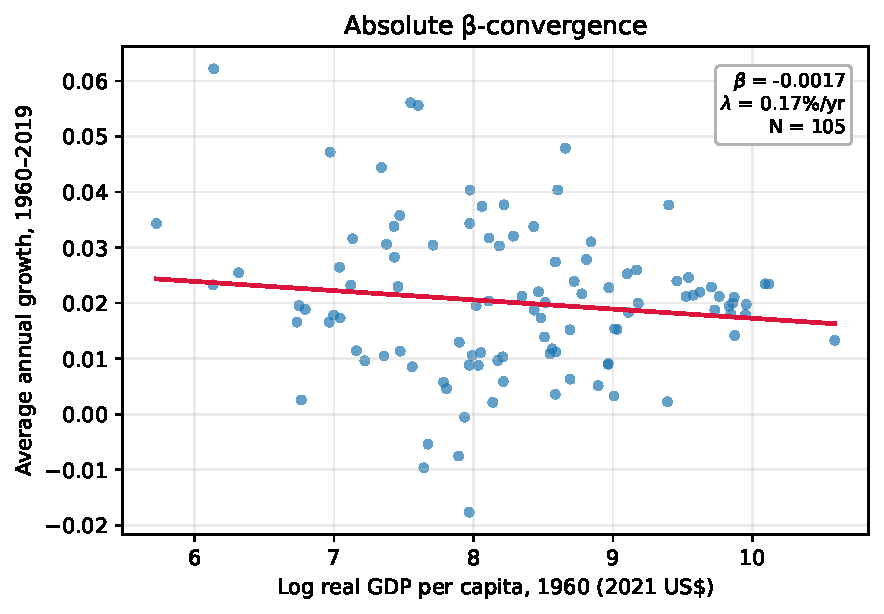
\includegraphics[width=0.72\textwidth]{beta_convergence.pdf}
  \caption{Absolute $\beta$-convergence: average annual growth against log
  initial GDP per capita. The fitted slope is flat.}
  \label{fig:beta}
\end{figure}

The dispersion evidence tells the same story. Figure~\ref{fig:sigma} plots the
cross-country standard deviation of log GDP per capita over time. Far from
falling, it \emph{rose} from \sigmaStart{} in \startYear{} to \sigmaEnd{} in
\finalYear --- $\sigma$-\emph{divergence} rather than convergence.

\begin{figure}[htbp]
  \centering
  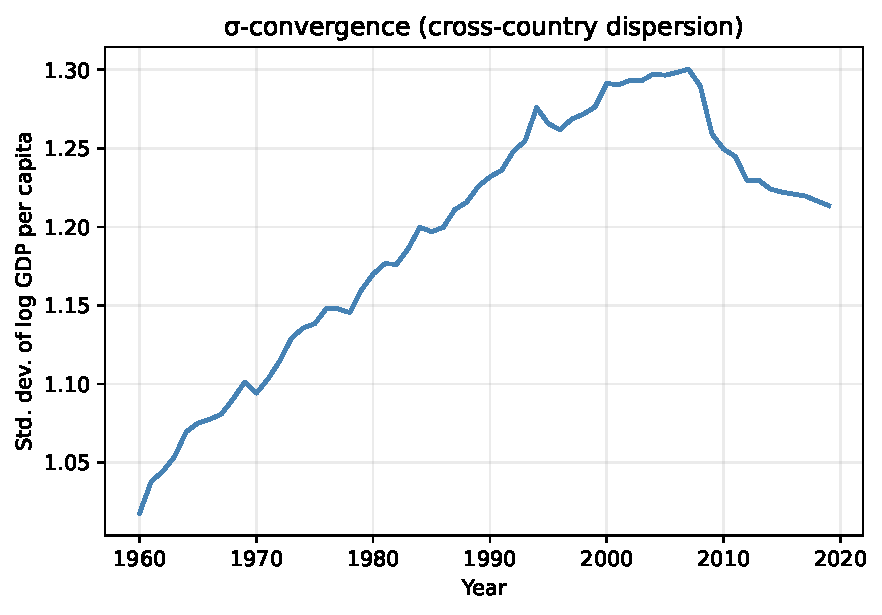
\includegraphics[width=0.72\textwidth]{sigma_convergence.pdf}
  \caption{$\sigma$-convergence: cross-country dispersion of log GDP per capita.
  Dispersion widens over the sample.}
  \label{fig:sigma}
\end{figure}

\section{Conclusions}
\label{sec:conclusions}
Across \Nabs{} economies from \startYear{} to \finalYear, we find neither absolute
$\beta$-convergence nor $\sigma$-convergence: poorer countries did not, on
average, grow systematically faster, and the world income distribution did not
compress. This is the well-known failure of \emph{unconditional} convergence.
The Solow model does not actually predict unconditional catch-up --- it predicts
convergence toward each economy's \emph{own} steady state. Testing that
conditional prediction, by controlling for the determinants of the steady state
(investment, population growth, and human capital), is the natural next step.

\bibliographystyle{apalike}
\bibliography{references}

\end{document}
